\documentclass[style=aggie]{powerdot}

\usepackage[utf8]{inputenc}

\pdsetup{}

\title{bioremediation and the cracked crystall ball}
\author{Stephan Richter}
\date{2013-04-30}

\begin{document}
\maketitle

\begin{slide}{Overview}
\tableofcontents[content=sections]
\end{slide}

\section{Motivation}
\begin{slide}{Situation}
\begin{itemize}
 \item many former industrial sites
 \item toxic pollutants sept into the soil for years/decades
 \includegraphics[width=0.8\textwidth]{waggon.ps}
 \item substances still there, resist degradation
 \item for some substances: degraders known
\end{itemize}
\end{slide}

\begin{slide}{Idea: Faciliation of BIOREMEDIATION using MULTIPLE BACTERIAL SPECIES}
\begin{itemize}
 \item potential degrading bacteria known\\ (at least for some contaminants)
\end{itemize}

\end{slide}
\section{S2}

\begin{slide}{}
first slide in second section?
\end{slide}

\end{document}
